\section{Application: JavaScript}\label{sec:application}

We actualize our approach for the JavaScript programming language via $\tool$,
which performs $N$+1-version testing for modern JavaScript engines and
ECMAScript, the language specification describing the syntax and semantics of
JavaScript in a natural language.

\subsection{Seed Synthesizer}

To synthesize seed JavaScript programs, we implement two different
synthesizers: \textit{non-recursive synthesizer} and \textit{built-in function
synthesizer}.

\subsubsection{Non-Recursive Synthesizer}

\begin{algorithm}[t]
  \caption{Algorithm caption}
  \label{alg:algorithm-label}
  \begin{algorithmic}
    \STATE \inred{TODO}
    \IF{some condition is true}
      \STATE do some processing
    \ELSIF{some other condition is true}
      \STATE do some different processing
    \ELSE
      \STATE do the default actions
    \ENDIF
  \end{algorithmic}
\end{algorithm}

For example, consider the following syntax of \textit{ArrayLiteral} in ES11:
\begin{figure}[H]
  \centering
  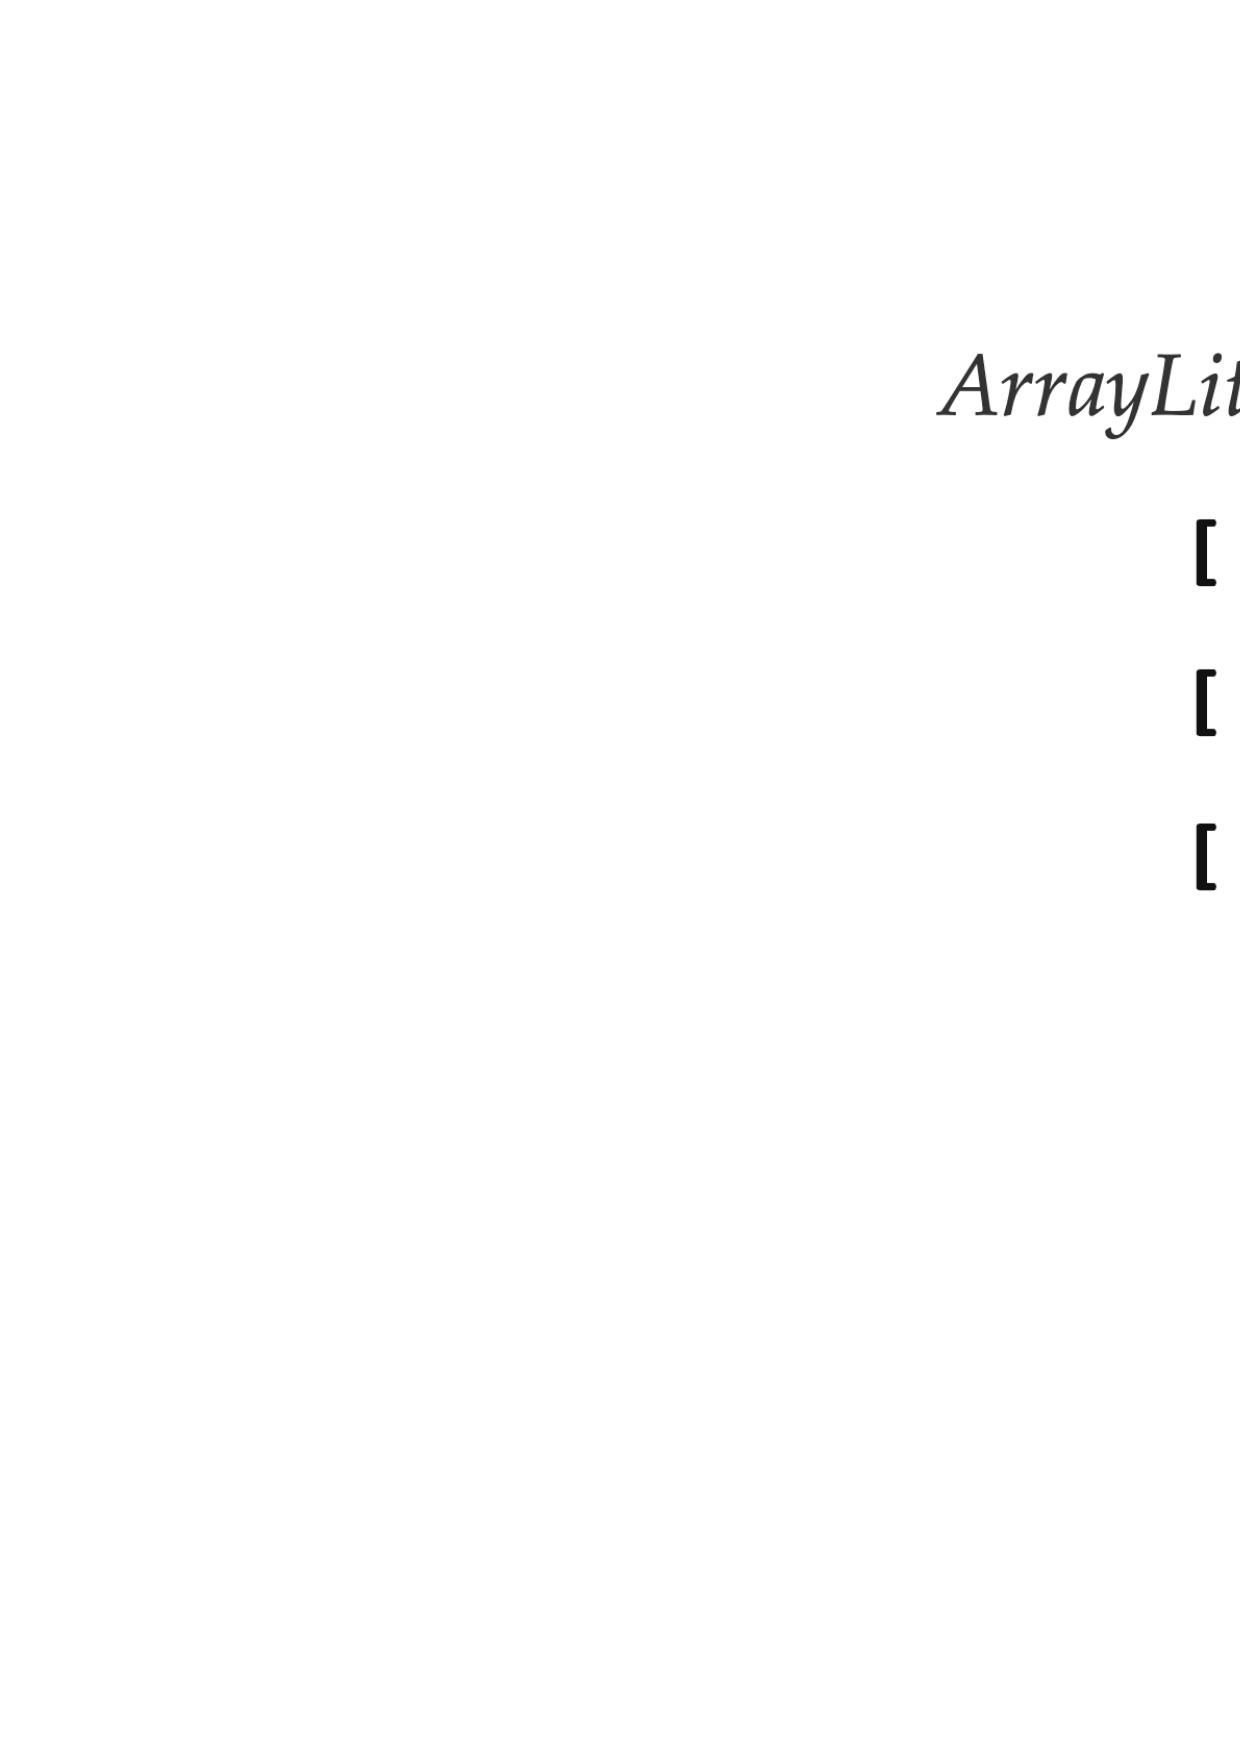
\includegraphics[width=0.42\textwidth]{img/syntax-arrayliteral.pdf}
\end{figure}

\inred{TODO}

\subsubsection{Built-in Function Synthesizer}
\inred{TODO}


\subsection{Target Selector}

\inred{TODO}


\subsection{Program Mutator}

\inred{TODO}


\subsection{Assertion Injector}

\inred{TODO}


\subsection{Bug Localizer}

\inred{TODO}
